%% Basierend auf einer TeXnicCenter-Vorlage von Tino Weinkauf.

\documentclass[a4paper,oneside,10pt]{report}
\usepackage[utf8]{inputenc}

\usepackage[backend=biber,citestyle=verbose,bibstyle=numeric,sorting=none]{biblatex}
\addbibresource{literatur.bib}

\usepackage{listings}
\usepackage{color}
\usepackage{xcolor}

\definecolor{dkgreen}{rgb}{0,0.6,0}
\definecolor{gray}{rgb}{0.5,0.5,0.5}
\definecolor{mauve}{rgb}{0.58,0,0.82}
\lstset{language=C++,
basicstyle=\ttfamily,
keywordstyle=\color{blue}\ttfamily,
stringstyle=\color{red}\ttfamily,
commentstyle=\color{gray}\ttfamily,
tabsize=2
}


\usepackage[ngerman]{babel}
%\usepackage[T1]{fontenc}
\usepackage[hidelinks]{hyperref}
\hypersetup{
	colorlinks=false,
	allcolors=black
}

%\usepackage{lmodern} 

\usepackage{graphicx}

\graphicspath{{images/}}    % Bilderverzeichnis


%% Packages für Formeln %%%%%%%%%%%%%%%%%%%%%%%%%%%%%%%%%%%%%
%\usepackage{amsmath}
%\usepackage{amsthm}
%\usepackage{amsfonts}



\begin{document}

\pagestyle{empty} 

\title{Entwicklung eines Remote Method Invocation Systems}
\author{Emil Watz, 5AHIF \protect\\Beispielnummer: 44 \protect\\Matrikelnummer: 19}
\maketitle
\tableofcontents 
\cleardoublepage 

\pagestyle{plain} 


\chapter{Theoretischer Hintergrund}

Das Ziel dieses Projekts ist die Entwicklung eines RMI-Systems basierend auf der \texttt{asio}-Bibliothek\footnote{\url{https://think-async.com/Asio/}} in \texttt{C++}. Im Folgenden werden ähnliche Systeme und Konzepte beschrieben. Daraus werden dann die Anforderungen an das System abgeleitet.  

\section{Was ist ein RMI-System}

Remote Method Invocation - auch Remote Procedure Call (RPC) genannt - beschreibt den Aufruf von "`entfernten Funktionen"', also Methoden die von einem anderen Prozess ausgeführt werden. Dieser Prozess muss jedoch nicht am gleichen Rechner ausgeführt werden. Im Kontext von verteilten Systemen werden die Prozesse meist von Rechnern in unterschiedlichen Netzwerken ausgeführt. Das bedeutet, dass Funktionsaufrufe und Rückgabewerte serialisiert, und über das Netzwerk übertragen werden müssen. 


\section{Zusammenhang mit Client/Server-Modell}

Das Konzept basiert auf dem Client/Server-Modell, bei dem der Client Anfragen sendet und der Server antwortet. Jedoch wird eine zusätzliche Abstraktion eingeführt. Der Client ruft eine lokale Funktion auf, die dem Server eine Anfrage sendet. Dieser führt eine Funktion aus und sendet den Rückgabewert serialisiert zurück. Dabei verhält sich der Aufruf am Client (in der Theorie) genau gleich wie ein lokaler Aufruf. 

\section{RMI-Konzept}

Es gibt kein allgegenwärtiges RMI-Protokoll oder einen Standard, jedoch haben viele Implementierungen eine ähnliche Struktur. 

\subsection{Allgemeines Konzept}

\begin{figure}
	\centering
	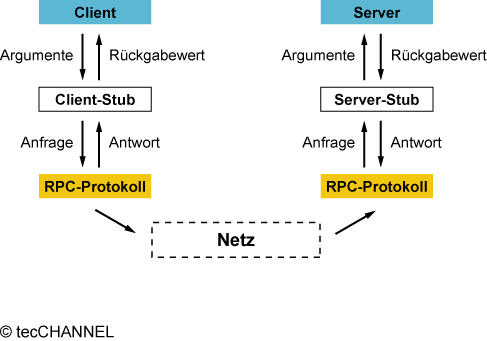
\includegraphics{microsoft_rpc}
	\caption[]{RPC-Prinzip\footnotemark}
	\label{fig:rpc}
\end{figure}

\footnotetext{\url{https://docs.microsoft.com/de-de/previous-versions/dn151205(v=technet.10)}}

Wie in der Abbildung zu sehen ist, gibt es im Grunde 3 "`Schichten"'. 
\begin{enumerate}
	\item Die oberste ist der Client und der Server. Sie sind die Anwender des Systems. Der Client ruft Funktionen am Server über den Client-Stub auf und gibt Argumente mit. Er kümmert sich aber nicht darum, wie die Aufrufe zum Server kommen. Der Server definiert die Funktionen, die vom Client aufgerufen werden können. Er gibt Rückgabewerte zurück, ist aber nicht dafür zuständig, wie diese zum Client kommen. Je nach Implementierung können auch Exceptions geworfen werden, diese werden in diesem Modell jedoch vernachlässigt
	\item Eine Ebene darunter befindet sich der Client- und Server-Stub. Sie sind für die Serialisierung und Deserialisierung der Argumente und Rückgabewerte zuständig.
	\item Die serialisierten Daten der Stubs werden dann von dem RPC-Protokoll über das Netzwerk übertragen, sodass sie wieder deserialisiert werden können\footcite{microsoft}. 
\end{enumerate}

\subsection{Java-RMI}

Eine konkrete Implementierung des, im vorherigen Abschnitt beschriebenem, Konzepts ist die Java-proprietäre Remote Method Invocation. Erweitert wird es durch einen Namensdienst, die sogenannte Registry, bei dem Objekte angemeldet und abgefragt werden können. Außerdem orientiert sich das Java-RMI an dem Proxy-Design-Pattern, welches im Folgenden beschrieben wird. 

\section{Das Proxy-Pattern}

Das Proxy-Pattern - auf Deutsch Stellvertreter-Entwurfsmuster - ist ein Design Pattern mit dem Ziel, einen Platzhalter für ein anderes Objekt bereitzustellen. So lässt sich der Zugriff auf das Objekt kontrollieren. Wie in Abbildung \ref{fig:proxy} zu sehen ist, besteht das Pattern grundlegend aus Komponenten. Der Platzhalter und das echte Objekt erben von einem Interface, welches die Methoden vorgibt. Beim Aufruf einer Funktion des Proxys, leitet dieser den Aufruf an das echte Objekt weiter\footcite[vgl.][Seite 207]{DesignPatterns}. 

\subsection{Proxy-Pattern im Kontext von RMI}

In einem RMI-System stellt der Client-Stub den Proxy beziehungsweise Stellvertreter dar. In diesem Fall handelt es sich um einen \textbf{remote proxy}, also einen lokalen Stellvertreter für ein Objekt in einem anderen Addressraum\footcite[vgl.][Seite 208]{DesignPatterns}. Das echte Objekt wäre in Abbildung \ref{fig:rpc} der Server. Die Weiterleitung eines Funktionsaufrufes ist bei einem RMI-System schwerer als bei einer rein lokalen Implementierung, da das "`echte Objekt"' von einem anderen Prozess instanziert wird und der Aufruf über Netzwerk übertragen werden muss. 

\begin{figure}
	\centering
	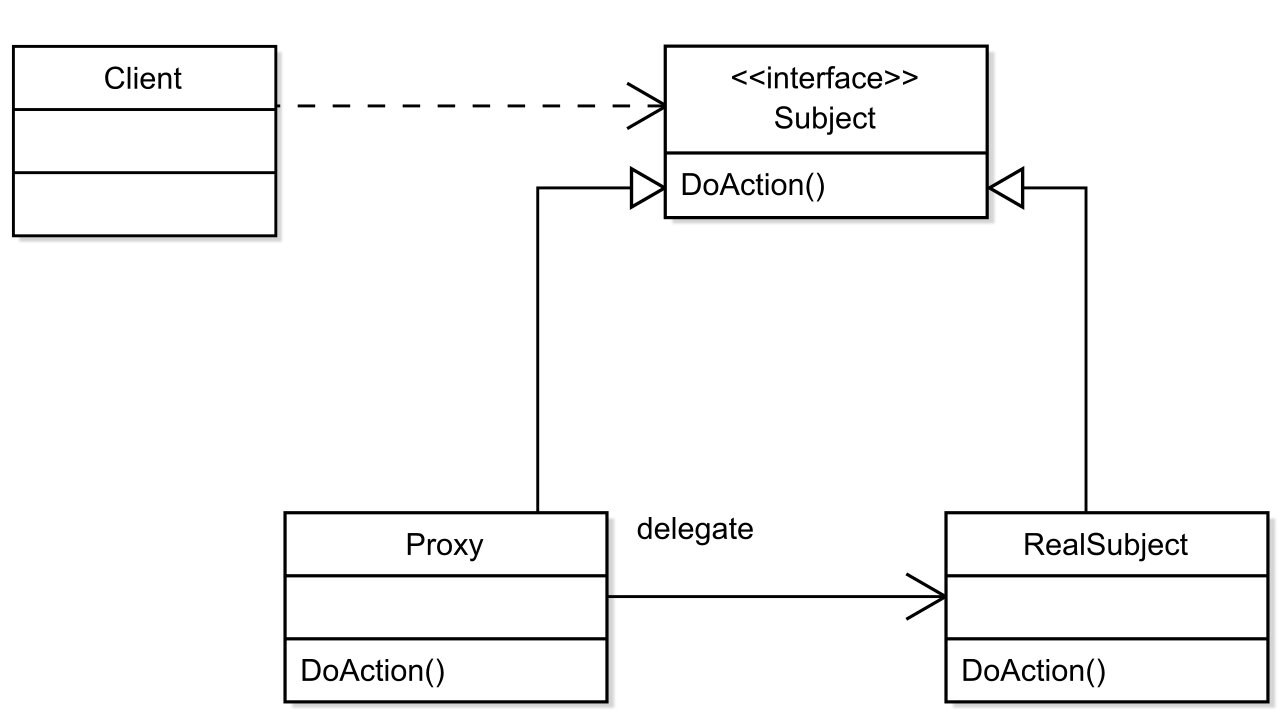
\includegraphics[width=12cm]{proxy_diagram}
	\caption[]{Simples Klassendiagram des Proxy-Patterns\footnotemark}
	\label{fig:proxy}
\end{figure}

\footnotetext{\url{https://www.programmingwithwolfgang.com/proxy-pattern-in-net-core/}}

\section{Anforderungen an ein RMI-System}

Auf Basis der bisher beschriebenen Informationen soll ein RMI-System implementiert werden. Die Anforderungen werden nun im Folgenden beschrieben. 

\subsection{Entferntes Aufrufen}

Ein Client soll einen \textbf{Remote-Proxy} in Form eines Client-Stubs instanzieren können, der die Methoden eines Interfaces implementiert. Beim Aufruf einer Methode wird der Aufruf über das Netzwerk gesendet. Die Methode wird dann am Server, der dasselbe Interface implementiert, aufgerufen. Dabei muss es die Möglichkeit geben, Parameter mitzusenden. Nachdem die Funktion am Server ausgeführt wurde, muss der Rückgabewert wieder zurückgesendet werden.  

\subsection{Exceptions}

Funktionen am Server können auch Exception werfen. Daher müssen diese ebenfalls an den Client-Stub zurückgesendet werden und dort geworfen werden.

\chapter{Umsetzung}

\section{Klassendiagram}

\begin{figure}[h]
\centering
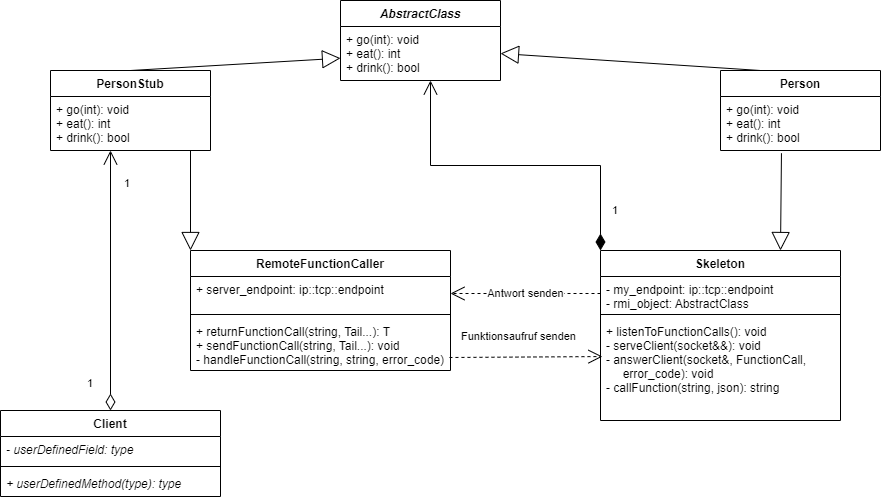
\includegraphics[width=12cm]{class_diagram}
\caption[My Caption]{Klassendiagram des RMI Systems}
\end{figure} 

Auf Basis der gesammelten Informationen aus dem letzten Kapitel wurde ein Klassendiagramm entwickelt. Dieses soll ein RMI-System anhand des Proxy-Patterns darstellen.

Die Klasse \texttt{Person} ist dabei ein Beispiel. Diese wird, genauso wie die Methoden der \texttt{AbstractClass}, vom Benutzer erstellt und kann auch anders heißen. Genauso ist es beim PersonStub. Die Verwendung dieses Systems wird in einem späteren Kapitel (\ref{verwendung}) genauer beschrieben. 


\subsection{Abstrakte Klasse (AbstractClass)}

Wie im Abschnitt über das Proxy-Pattern beschrieben, implementieren die Klassen ein Interface, welches die Methoden definiert, die über das Netzwerk aufgerufen werden können. 

\subsubsection{\texttt{C++} Implementierung} \label{abstractClass}

Da es in \texttt{C++} an sich keine Interfaces gibt, wird eine abstrakte Klasse mit dem Namen \texttt{AbstractClass} verwendet. Die Methoden der Klasse werden mit dem \texttt{virtual}-Schlüsselwort gekennzeichnet. Dadurch können sie von einer abgeleiteten Klasse überschrieben werden. Mit dem setzen auf 0 werden daraus "`pure-virtual functions"', die überschrieben werden \textbf{müssen}.
\begin{lstlisting} 
class AbstractClass {
  public:
	virtual ~AbstractClass() { }
	virtual void go(int i) = 0;
	virtual bool drink() = 0;
	virtual int eat() = 0;
};
\end{lstlisting}

Die Methodendeklarationen können nach Belieben geändert werden. Der Name der Klasse und der Destruktor müssen jedoch wie vorgegeben verwendet werden.

\subsection{Server-Objekt / \texttt{Person}-Klasse}

In dem Klassendiagramm wird für das Server-Objekt als Beispiel die \texttt{Person}-Klasse verwendet. Diese Klasse enthält die eigentliche Logik, die über das Netzwerk aufgerufen werden soll. Sie erbt ebenfalls von der abstrakten Klasse, kann aber vom Benutzer frei gestaltet werden, solange sie die vorgegebenen Methoden implementiert. 

\subsection{PersonStub}

Die Client-Stub-Klasse erbt von der abstrakten Klasse. Die Implementierungen der virtuellen Funktionen, senden einen Funktionsaufruf an die Skeleton-Klasse des Servers. Den Rückgabewert oder die Exception erhält der Client-Stub in serialisierter Form wieder vom Skeleton. 

Der \texttt{PersonStub} ist der Stellvertreter für die \texttt{Person}-Klasse. Er ist das Equivalent zum Client-Stub. 

Da der Client-Stub von \texttt{AbstractClass} abgeleitet wird, müssen die Funktionen überschrieben werden. Der \texttt{PersonStub} ist dafür da, um den Funktionsaufruf samt Parameter an den \texttt{RemoteFunctionCaller} zu übergeben. Um die Verwendung zu vereinfachen, wurden dafür 2 Makros erstellt. 

\subsubsection{\texttt{C++} Implementierung}

\begin{lstlisting}
//Zeilenumbrueche nur damit die Zeile nicht zu lange ist
#define __SEND_FUN__(type, ...) 
return RemoteFunctionCaller::returnFunctionCall<type>
		(__func__, __VA_ARGS__);

#define __SEND_VOID_FUN__(...) 
RemoteFunctionCaller::sendFunctionCall(__func__, __VA_ARGS__);
\end{lstlisting}


Es gibt zwei unterschiedliche Makros. Der \texttt{\_\_SEND\_FUN\_\_}-Makro wird verwendet, wenn es einen Rückgabewert gibt. In dem Fall ist der erste Parameter der Rückgabewert und danach kommen die Parameter. Der Makro ruft das \texttt{returnFunctionCall}-Template auf. Dabei wird der Typ als Template-Parameter mitgegeben. Das erste "`normale"' Argument ist ein weiterer Makro \texttt{\_\_func\_\_}, der den aktuellen Funktionsname als \texttt{char[]} einfügt. \texttt{\_\_VA\_ARGS\_\_} fügt die weiteren Argumente, getrennt mit einem Beistrich, ein. 

Bei Funktionen ohne Rückgabewert muss der Makro \texttt{\_\_SEND\_VOID\_FUN\_\_} verwendet werden. Dieser Makro ruft die \texttt{sendFunctionCall}-Funktion auf und macht dasselbe wie der andere Makro, jedoch muss kein Typ angegeben werden. 


\subsection{Der \texttt{RemoteFunctionCaller}}

Diese Klasse ist für die Serialisierung, das Senden des Funktionsaufrufes und die Deserialisierung des Rückgabewertes zuständig. Wie schon im Teil über den \texttt{PersonStub} beschrieben, werden, je nachdem ob es einen Rückgabewert gibt oder nicht, entweder die \texttt{returnFunctionCall}- oder die \texttt{sendFunctionCall}-Funktion aufgerufen. 

\subsubsection{\texttt{returnFunctionCall}}

Beide davon sind Funktionstemplates. Im Gegensatz zur \texttt{sendFunctionCall}-Methode, muss jedoch bei dieser Funktion, der Rückgabewert angegeben werden. Dieser wird durch den \texttt{typename T} bestimmt und wird als Template-Argument in den spitzen Klammern übergeben. Die Parameter bestehen zuerst aus dem Namen der Funktion, die aufgerufen werden soll. Außerdem wird ein \texttt{Parameter-Pack} verwendet. Dadurch kann eine variable Anzahl an Argumenten mit unterschiedlichen Typen entgegengenommen werden. 

\begin{lstlisting}
template<typename T, typename... Tail>
T returnFunctionCall(std::string name, Tail... tail);
\end{lstlisting}

\subsubsection{\texttt{sendFunctionCall}}

\begin{lstlisting}
template<typename... Tail>
void sendFunctionCall(std::string name, Tail... tail);
\end{lstlisting}

\texttt{sendFunctionCall} ist sehr ähnlich zur anderen Funktion. Es wird ebenfalls ein \texttt{Parameter-Pack} verwendet, jedoch kann kein Return-Typ angegeben werden und es wird nichts zurückgegeben. 

\subsubsection{Serialisierung}

Die Serialisierung der Parameter erfolgt über die \texttt{JSON for modern C++}-Bibliothek\footnote{\url{https://github.com/nlohmann/json}}. Außerdem wird wieder ein variadisches Template verwendet. Das \texttt{Parameter-Pack} wird an die \texttt{convertParametersToJson}-Methode weitergegeben. 

\begin{lstlisting}
template<typename T>
void convertParametersToJson(nlohmann::json& j, int& i, T last) {
    i++;
    j[std::to_string(i)] = last;
}


template<typename T, typename... Tail>
void convertParametersToJson(nlohmann::json& j, int& i, 
  T head, Tail... tail) {
    i++;
    j[std::to_string(i)] = head;
    convertParametersToJson(j, i, tail...);
}
\end{lstlisting}

Der erste Parameter ist eine Referenz auf ein Json-Objekt. Der zweite ist ein Integer, der die Stelle des Parameters bestimmt. Die Methode wird so lange rekursiv aufgerufen, bis nur mehr ein Parameter übrig ist. Dann wird mit einer überladenen Funktionen der letzte Parameter in das Json-Objekt eingefügt. 

Der, durch den \texttt{\_\_func\_\_}-Makro serialisierte, Name der Funktion und das Json-Objekt mit den Parametern wird dann an die \texttt{handleFunctionCall}-Funktion weitergegeben. Diese kümmert sich um die Übertragung des Funktionsaufrufes und Empfangen des Rückgabewertes/der Exception. Die Kommunikation wird im Abschnitt \ref{kommunikation} noch genauer beschrieben. 

\subsection{\texttt{Skeleton}-Klasse}

Diese Klasse ist für Deserialisierung des Funktionsaufrufes und Serialisierung des Rückgabewertes oder der Exception zuständig. Sie hat eine Instanz \texttt{rmi\_object} einer \texttt{AbstractClass}. Die Skeleton-Klasse ruft die entsprechenden Funktionen an dieser Instanz auf, wenn ein Funktionsaufruf von einem Client ankommt. Dazu müssen die Aufrufe deserialisiert werden. Das geschieht folgendermaßen:  

\subsubsection{Deserialisierung}

Für die Deserialisierung werden wieder Makros eingesetzt. Sie werden in der \texttt{skeleton.h}-Datei definiert. 

\begin{lstlisting}
//Zeilenumbrueche damit die Zeile nicht zu lange ist
#define __ARGUMENT__(type, place) par[#place].get<type>()

#define __FUNCTION__(name, ...) 
if (functionName == #name) {
	service.incrementCounter(#name); 
	j["returnValue"] = rmi_object->name(__VA_ARGS__);
}

#define __VOID_FUNCTION__(name, ...) 
if (functionName == #name) {
	service.incrementCounter(#name); 
	rmi_object->name(__VA_ARGS__);
}

#define __END__ return j.dump();
\end{lstlisting}

Es wird wieder zwischen Funktionen mit und ohne Rückgabewerten unterschieden. Jeder Parameter muss mit dem \texttt{\_\_PARAMETER\_\_}-Makro angegeben werden. Dabei muss der Typ und die Position des Parameters angegeben werden. Das ist notwendig, damit der Parameter an der richtigen Stelle und mit dem richtigen Datentypen aus dem Json-Objekt ausgelesen werden kann. Nachdem die Funktion ausgeführt wurde, wird ein neues Json-Objekt mit (oder ohne) dem Rückgabewert als String zurückgegeben. 

In der \texttt{abstractMethods}-Datei wird die \texttt{callFunction} mit den Makros definiert. Eine Beispielangabe ist im Abschnitt \ref{abstractMethods} zu finden. 

\section{Kommunikation mit Protokoll Buffers} \label{kommunikation}

Die Kommunikation zwischen dem \texttt{RemoteFunctionCaller} und dem \texttt{Skeleton} basiert auf Google Protokoll Buffers.  

\subsection{Protokoll Buffer Definitionen}

Im Rahmen des Projekts werden 2 unterschiedliche Protokoll Buffer verwendet. Der erste ist für den Funktionsaufruf. 

\subsubsection{Funktionsaufruf}

\begin{lstlisting}
syntax = "proto3";

message FunctionCall {
  string name = 1;
  optional string json_arguments = 2;
}
\end{lstlisting}

Im der \texttt{FunctionCall}-Nachricht wird der Name der Funktion gespeichert und die Argumente als Json-String. Die Argumente sind logischerweise als optional gekennzeichnet, da nicht jede Funktion Parameter hat. 

\subsubsection{Rückgabewert}\label{proto:returnvalue}

Bei der \texttt{ReturnValue}-Nachricht wird zuerst gespeichert, ob der Funktionsaufruf erfolgreich ausgeführt werden konnte. Dadurch können auch \texttt{void}-Funktionen bestätigt werden. Zusätzlich wird entweder ein String mit dem Rückgabewert als Wert im Json-Format gespeichert. Oder es wird die Nachricht einer Exception gespeichert, die geworfen wurde. 

\begin{lstlisting}
syntax = "proto3";

message ReturnValue {
  bool success = 1;
  optional string json_value = 2;
  optional string exception_text = 3;
}
\end{lstlisting}

\subsubsection{Übertragung}

Nachdem die Protokoll Buffer erstellt wurden, müssen sie übertragen werden. Die Übertragung wird von dem \texttt{RemoteFunctionCaller} und dem \texttt{Skeleton} übernommen. Für das Senden gibt es jeweils eine \texttt{sendProtoBuffer}-Funktion. Diese legt einen \texttt{asio::streambuf}, der für die Kommunikation verwendet wird. Da das Ende eines Protokoll Buffers nicht markiert wird, muss der Empfänger die Länge wissen. Darum werden zuerst 4 Bytes im \texttt{streambuf} reserviert, welche die Länge (\texttt{ByteSizeLong}) speichern. Nachdem diese gesendet werden, wird der Protokoll Buffer zu einem \texttt{ostream} serialisiert und mit dem Socket versendet. 

\begin{lstlisting}
//Verkuerzte Version der Serialisierung im RemoteFunctionCaller
asio::streambuf buf;
buf.prepare(4);
std::ostream os(&buf);
uint32_t protobufLength = f->ByteSizeLong();
os << protobufLength;
buf.commit(4 - buf.size());
size_t serializeSuccessful = f->SerializeToOstream(&os);
asio::write(sock, buf.data(), ec);
\end{lstlisting}

Am anderen Ende der Verbindung werden dann zuerst die 4 Bytes mit der Länge n gelesen. Danach werden die n Bytes gelesen, und von einem \texttt{istream} in ein Objekt deserialisiert.

\begin{lstlisting}
//Deserialisierung im Skeleton
read(sock, buf.prepare(4), ec);
...
asio::read(sock, buf.prepare(protobufLength), ec);
...
functionCall->ParseFromIstream(&is)
\end{lstlisting}

\section{Exceptions}

Es kann natürlich auch sein, dass die Funktion am Server gar keinen Rückgabewert zurückliefert, sondern eine Exception wirft. In diesem Fall muss diese auch über das Netzwerk zurückgesendet werden. Wie schon im Abschnitt \ref{proto:returnvalue} beschrieben, gibt es ein optionales Feld für die Exception-Nachricht. Die \texttt{callFunction}-Methode wird in einem \texttt{try/catch}-Block ausgeführt. Wenn eine Exception geworfen wird, wird das \texttt{exception\_text}-Feld mit der Exception-Nachricht gesetzt. 

\begin{lstlisting}
try {  
	std::string s{callFunction(d->name(), j)};
	returnValue->set_json_value(s);
} catch (const std::exception& ex) {
	spdlog::info("Funktion " + d->name() + 
		" hat eine Exception geworfen: " + ex.what());
	returnValue->set_exception_text(ex.what());
}
\end{lstlisting}

Wenn der Protokoll Buffer am Client ankommt, wird mit der \texttt{has\_exception\_text()}-Methode überprüft, ob das Exception-Feld gesetzt ist. Wenn ja, wird eine \texttt{rmi\_user\_error} geworfen, welche die Nachricht des Feldes enthält.

\begin{lstlisting}
//r => ReturnValue
if (r->has_exception_text()) {
	spdlog::info("Ein Fehler wurde geworfen: " + 
		r->exception_text());
	const std::string s{r->exception_text()};
	delete r;
	throw rmi_user_error(s);
}
\end{lstlisting}

\section{Fehlerbehandlung}

Die Fehlerbehandlung basiert größtenteils auf Fehlercodes (\texttt{asio::error\_code}). Nach einer Operation, die einen Fehler erzeugen kann, wird überprüft, ob der Wert des Fehlercodes 0 ist. Wenn nicht wird eine Fehlermeldung mit \texttt{spdlog} ausgegeben und die Funktion bricht ab. Im Folgenden Codestück wird eine beispielhafte Fehlerbehandlung in der \texttt{handleFunctionCall}-Funktion gezeigt:

\begin{lstlisting}
sock.connect(server_endpoint, ec);
if (eclog::error("Verbindung zu " + 
	server_endpoint.address().to_string()\
	+ " konnte nicht aufgebaut werden", sock, ec)) 
return nullptr;
\end{lstlisting}

Im \texttt{error\_handler.h} sind (im Namespace \texttt{eclog}) Funktionen definiert, welche die Fehlerbehandlung vereinfachen. Wenn der Fehlercode gesetzt ist, wird die Fehlermeldung ausgegeben, und es wird \texttt{true} zurückgeliefert. In diesem Fall schließt die Überladung der Funktion sogar den Socket. Danach wird die Funktion abgebrochen indem der \texttt{nullptr} zurückgegeben wird. Der \texttt{error\_code ec} ist ein Referenzparameter, dadurch weiß die aufrufende Funktion ebenfalls, dass ein Fehler aufgetreten ist. 

Wenn ein Fehler bei der Übertragung auftritt, wird der Fehlercode solange propagiert, bis er bei der \texttt{returnFunctionCall/sendFunctionCall}-Funktion ankommt. Dort wird die \texttt{rmi\_system\_error}-Exception geworfen. Dadurch wird dem Benutzer mitgeteilt, dass der Aufruf fehlgeschlagen ist. 

\section{gPRC}

Das RMI-System wurde durch einen Server erweitert, über den Statistiken abgefragt werden. Dieser wurde mittels gRPC implementiert.

\subsection{Proto-Definition}

Der RPC-Service wird via Protokoll Buffer in der \texttt{statistics\_server.proto}-Datei folgendermaßen definiert.

\begin{lstlisting}
service StatisticsManager {
  rpc GetStatistics (StatsRequest) returns (StatsReply) {}
  rpc GetFunctionNames (google.protobuf.Empty) 
				returns (FunctionNamesReply) {}
}

message StatsRequest {
  string function_name = 1;
}

message StatsReply {
  int32 counter = 1;
}

message FunctionNamesReply {
  string names = 1;
}
\end{lstlisting}

Es wird ein StatisticsManager-Service definiert, der zwei Funktionen hat. GetStatistics hat den Parameter StatsRequest, der den Namen einer Funktion enthält. Die Funktion liefert die Anzahl der Aufrufe dieser Funktion zurück. Die Funktion GetFunctionNames hat keinen Parameter. In gRPC muss jede Funktion jedoch einen Parameter haben, weswegen hierfür der zur Verfügung gestellte Protokoll Buffer \texttt{google.protobuf.Empty} verwendet wird. Der Rückgabewert enthält die Namen aller Funktionen, die über das RMI-System aufgerufen werden können.

\subsection{Umsetzung}

Die durch gRPC generierten Klassen werden durch die Klassen \textbf{StatisticsManagerImpl} und \textbf{StatisticsManagerClient} erweitert. 

\subsubsection{StatisticsManagerImpl}

Diese Klasse stellt den gRPC-Server dar. Sie erbt von dem gRPC-generierten StatisticsManager::Service und implementiert die Methoden. 

\begin{lstlisting}
class StatisticsManagerImpl final : public StatisticsManager::Service {
...
  public: 
    grpc::Status GetStatistics(grpc::ServerContext* context, 
			const StatsRequest* request,
			StatsReply* reply) override;
    grpc::Status GetFunctionNames(grpc::ServerContext* context, 
			const ::google::protobuf::Empty* request,
      FunctionNamesReply* reply) override;
...
}
\end{lstlisting}

Die Skeleton-Klasse hat eine Instanz des StatisticsManagerImpl. In einem eigenen Thread wird in der Funktion \texttt{startStatisticsManager} ein Server mit dieser Instanz gestartet. Dabei wird der Port 50051 verwendet.

\subsubsection{StatisticsManagerClient}

Die Klasse ist ein Wrapper für den StatisticsManager::Stub. Sie hat ebenfalls die zwei gRPC-Funktionen, welche den Aufruf an den Stub weiterleiten. Dabei werden die Parameter in den entsprechenden Protokoll Buffer umgewandelt beziehungsweise der Returnwert aus dem Protokoll Buffer ausgelesen und zurückgegeben.

\begin{lstlisting}
class StatisticsManagerClient {
  public: 
    StatisticsManagerClient(std::shared_ptr<grpc::Channel> channel)
      : stub_(StatisticsManager::NewStub(channel)) {}
    int GetStatistics(const std::string&);
    std::string GetFunctionNames();
  private:
    std::unique_ptr<StatisticsManager::Stub> stub_;
};
\end{lstlisting}

Der Client kann diese über den RemoteFunctionCaller (und dadurch auch über den Stub) aufrufen. Der RemoteFunctionCaller hat eine Instanz des StatisticsManagerClient und ebenfalls die Funktionen \texttt{GetStatistics} und \texttt{GetFunctionNames}, die den Aufruf an die Instanz weiterleiten. 

\chapter{Verwendung} \label{verwendung}

In diesem Kapitel wird beschrieben, wie das RMI-System verwendet wird und wie es konfiguriert werden kann. 

Die Ordnerstruktur ist folgendermaßen aufgebaut: Im \texttt{src}-Ordner befinden sich drei Ordner. Der erste ist der \texttt{client}-Ordner. In diesem kann der Client vom Anwender implementiert werden. Der \texttt{rmi}-Ordner ist für die \texttt{skeleton.cpp} vorgesehen, dieser darf nicht verändert werden. Im \texttt{server}-Ordner ist die \texttt{abstractMethods}-Datei, welche die serverseitigen Funktionsdeklarationen enthält. In dem Ordner kann außerdem der Server entwickelt werden. 

Der \texttt{include}-Ordner enthält den Ordner \texttt{rmi\_user}. In diesem ist die \texttt{abstractClass} und die \texttt{.h}-Dateien für das Server-Objekt (Person) und den Stub (PersonStub). Der \texttt{rmi\_system}-Ordner enthält Dateien, die für das System notwendig sind, aber nicht verändert werden dürfen. 

\section{Konfiguration der Methoden}

Damit die Funktionen aufgerufen werden können, müssen diese in verschiedenen Orten angegeben werden. 


\paragraph{AbstractClass} Diese muss in der \texttt{abstractClass.h}-Datei "`pure-virtual"' Funktionsdefinition enthalten. Beispiel: \ref{abstractClass}
\paragraph{Server-Objekt} Das Server-Objekt muss von der AbstractClass und dem Skeleton erben und die Funktionen der AbstractClass überschreiben. Es kann sonst frei gestaltet werden. Wichtig ist, dass im Konstruktor der Skeleton-Konstruktor aufgerufen wird mit dem Pointer auf das aktuelle Objekt (\texttt{this}). Damit Anfragen des Clients vom Server verarbeitet werden, muss die Funktion \texttt{listenToFunctionCalls} des Skeletons aufgerufen werden. Diese Funktion horcht auf Anfragen auf dem \textbf{Port 50113}. Im folgenden Beispiel wird sie im Konstruktor von \texttt{Person} aufgerufen.

\begin{lstlisting}
class Person : public AbstractClass, public Skeleton {
  public:
    Person() : Skeleton(this) {
      listenToFunctionCalls();
    }
    ~Person() { };
    void go(int i);
    int eat();
    bool drink();
};
\end{lstlisting}

\paragraph{Client-Stub} Dieser sollte im \texttt{rmi\_user}-Ordner definiert werden. Die Klasse muss von der AbstractClass und dem RemoteFunctionCaller erben. Dabei muss jede Funktion definiert werden mit dem \texttt{\_\_SEND\_FUN\_\_} oder \texttt{\_\_SEND\_VOID\_FUN\_\_}-Makro. Bei beiden müssen die Parameter angegeben werden, wobei bei dem ersten Makro noch der Rückgabewert als erstes Argument angegeben werden muss. 

\begin{lstlisting}
class PersonStub : public AbstractClass, RemoteFunctionCaller {
  public:
    void go(int i) {
        __SEND_VOID_FUN__(i)
    }

    int eat() {
        __SEND_FUN__(int)
    }

    bool drink() {
        __SEND_FUN__(bool)
    }
};
\end{lstlisting}

Beim Aufruf senden diese Funktionen eine Anfrage auf den \textbf{(TCP-)Port 50113 des lokalen Hosts}.

Außerdem müssen dafür die \texttt{abstractClass.h} und \texttt{remoteFunctionCaller.hpp}-Dateien inkludiert werden. 

\paragraph{Skeleton-Definitionen} \label{abstractMethods}

In der \texttt{abstractMethods}-Datei müssen die \texttt{\_\_FUNCTION\_\_} beziehungsweise \texttt{\_\_VOID\_FUNCTION\_\_}-Makros angegeben werden. Das erste Argument ist dabei der Name der Funktion und die restlichen Argumente müssen mit dem \texttt{\_\_PARAMETER\_\_}-Makro definiert werden. Dabei ist das erste Argument des Makros der Typ und der zweite die Position. Am Schluss muss noch der \texttt{\_\_END\_\_}-Makro aufgerufen werden. Eine beispielhafte Angabe sieht folgendermaßen aus: 

\begin{lstlisting}
std::string Skeleton::callFunction(const std::string functionName, 
  nlohmann::json par) {
    nlohmann::json j;
    __VOID_FUNCTION__(go, __ARGUMENT__(int, 1))
    __FUNCTION__(drink)
    __FUNCTION__(eat)
    __END__
}
\end{lstlisting}

\section{CLI}

Das RMI-System selbst kann nicht per CLI gesteuert werden, da der Einstiegspunkt in das Programm vom Anwender bestimmt wird. In der beispielhaften Anwendung wurde jedoch eine Kommandozeilenschnittstelle erstellt. Im der \texttt{main.cpp} des Server-Prozesses können folgende Einstellungen getroffen werden: 
\begin{lstlisting}
RMI Server
Usage: ./server [OPTIONS]

Options:
  -h,--help                   Print this help message and exit
  --loglevel UINT             Log level: 0 = fatal, 1 = error,
                              2 = warning, 3 = info
\end{lstlisting}

Mit dem \texttt{loglevel} wird bestimmt, bis zu welcher Stufe Meldungen ausgegeben werden. Der Standardwert ist dabei 3. 

\begin{lstlisting}
RMI Client
Usage: ./client [OPTIONS]

Options:
  -h,--help                   Print this help message and exit
  --loglevel UINT             Log level: 0 = fatal, 1 = error,
                              2 = warning, 3 = info
\end{lstlisting}

Die Schnittstelle des Clients ist im Grunde ident mit der des Servers. 

\addtocontents{toc}{\protect\vspace*{\baselineskip}}

%% Literaturverzeichnis
%% ==> Eine Datei 'literatur.bib' wird hierfür benötigt.
%% ==> Sie müssen hierfür BibTeX verwenden (Projekt | Eigenschaften... | BibTeX)
%\addcontentsline{toc}{chapter}{Literaturverzeichnis}
%\nocite{*} %Auch nicht-zitierte BibTeX-Einträge werden angezeigt.
%\bibliographystyle{alpha} %Art der Ausgabe: plain / apalike / amsalpha / ...
%\bibliography{literatur} %Eine Datei 'literatur.bib' wird hierfür benötigt.

%% Abbildungsverzeichnis
%%\clearpage
%%\addcontentsline{toc}{chapter}{Abbildungsverzeichnis}
%%\listoffigures

%% Tabellenverzeichnis
%%\clearpage
%%\addcontentsline{toc}{chapter}{Tabellenverzeichnis}
%%\listoftables


%%%%%%%%%%%%%%%%%%%%%%%%%%%%%%%%%%%%%%%%%%%%%%%%%%%%%%%%%%%%%
%% ANHÄNGE
%%%%%%%%%%%%%%%%%%%%%%%%%%%%%%%%%%%%%%%%%%%%%%%%%%%%%%%%%%%%%
%%\appendix
%% ==> Schreiben Sie hier Ihren Text oder fügen Sie externe Dateien ein.

%\input{Dateiname} %Eine Datei 'Dateiname.tex' wird hierfür benötigt.


\end{document}